\chapter{Preliminaries}
\label{chapter:preliminaries}

The following Sections describe all the concepts required for the reader to understand the proposed method in this thesis. However, it is still assumed that the reader has some basic knowledge about programming and computational intelligence. For this reason, the following concepts are focused on terms related to finance, specifically to trading and financial markets, and to agent-based models and multi-agent systems.

\section{Financial Market}
\label{section:financial-market}

A financial market is constructed by the interaction of a number of traders, where a trader is an entity that is able to buy or sell a number of units of an asset. The entities defined as traders can either be individual human beings, organizations or even computer programs. An asset can be anything that can be priced and can be divided so different parties can hold a share of the asset. For example, corn can be priced and different parties can hold a share of the corn market by physically owning corn. Lastly, traders can decide to either buy or sell shares of this asset. Although this decision can seem simple, as there can only be two outcomes, the process a trader can follow in order to arrive to an outcome can be very complex.

In theory, if one can know all the variables that each trader is taking into consideration to arrive to their particular decisions, the prices in a financial market can be precisely predicted. Obviously, this is impossible, unless we were simulating a financial market with a handful of people and everyone was telling everyone else what decisions they are going to take. Nevertheless, one can create models that closely simulate a financial market, and one can assume that these simulations are generalizations of the real financial market.

\section{Trading Strategy}
\label{section:trading-strategy}

A trading strategy is a set of processes that help a trader to determine different aspects of a financial market and to later make trading decisions based on these aspects. For example, a trader can determine that a market is going to follow an uptrend -- that is, that the price of a financial market is going to rise -- and take the decision of buying shares of the asset of that financial market. Trading strategies can vary in complexity: some can use simple moving averages to determine trends and entry points, and others can take into consideration many different indicators, as well as the trader's experience.

An untrained person can think that trading a financial market only involves deciding when to buy or sell a market. Nevertheless, the possible decisions can be as complex as the strategy used to determine them. For instance, when traders are about to open a new buy or sell order, they also need to decide the size of the order, or how many units are going to be bought or sold. These units can be shares in a stock market or an amount of a currency in foreign exchange markets, for example. This order can also be delayed: the trader can decide that an order will be opened when a certain amount of time passes or when certain price in a financial market is reached. Additionally, the trader can specify \textit{stop loss} and/or \text{take profit} prices: after executing a buy or sell order, if the market reaches certain price, the trade has to be cancelled, stopping any losses or taking any profits that that trade generated since it was created.

The initial process of creating a trade order is complex, as noted in the previous paragraph, but decisions can also take place after a number of trade orders have been executed. The most obvious decision is when one should stop a trade. This particular decision has spawned several psychological research works, where the decision process is analyzed. A clear example is depicted in Figure \ref{figure:trading-psychology}, where the emotions that traders generally feel when experiencing a the earnings or losses of a trade are shown.

%% Amaury: I will create my own version of this chart (re-make it to match style)
%% Amaury: I will also cite this
\begin{figure}
\caption{Trading psychology}
\centering
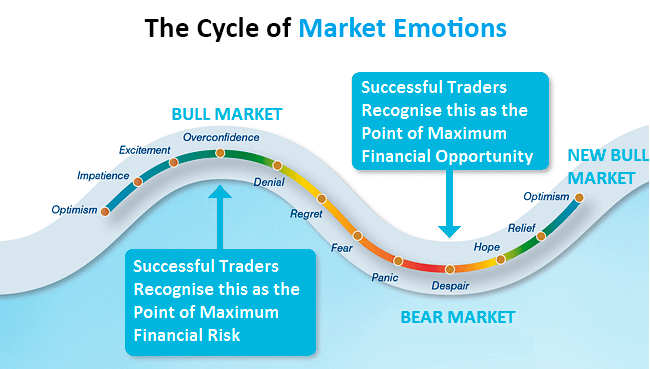
\includegraphics[width=1.0\textwidth]{img/trading-psychology.png}
\label{figure:trading-psychology}
\end{figure}

Stopping a trade does not only involve emotions, as a thorough analysis of the market, about the current's account financial situation and the trades themselves needs to be performed. Regarding about the first step -- an analysis of the market -- it is worth mentioning that these analyses are usually different than those performed when deciding when to start trading a market. For example, in a stagnated market one could decide not to trade a market, but this does not necessarily mean that one should close trade orders in this situation; one could consider that this is a moment where trades need to be held until further price movements take place. A trader can also decide to \textit{partially} stop a trade; that is, a trader can decide to sell a certain amount of units from a trade, for example. Likewise, a trader can decide to acquire more units from the asset.

It is usual that a trader \textit{diversifies} its trading portfolio. Diversifying means that a trader starts trading a number of financial markets instead of focusing on a single market. The advantages of this %% Amaury: \cite
are that the risk diminishes, as the profits of trading some markets can compensate the losses obtained from trading other markets. Diversification can then make trading strategies even more complex, as a trader now needs to take into consideration different markets. Additionally, markets usually affect the price movements of other markets, for example, if wheat price goes up, this can directly impact the price of McDonald's stock prices, as many of their products contain wheat-based ingredients. Furthermore, if McDonald's stock market is severely affected, this could negatively impact the United States' economy, as McDonald's is one of the most profitable companies in this country. Depending on the robustness of a trading strategy, all of these aspects can be considered to take a decision.

Trading strategies have existed since the activity of trading was created. To illustrate this, one can consider how the Japanese traded certain commodity markets, such as the rice market, using strategies based on candlestick patterns. %% Amaury: \cite
The Japanese charted the prices by representing the open, highest, lowest and close prices for a period of time using a figures that resemble candles and their wicks, as the ones seen in Figure \ref{figure:candlestick-chart}. The body of a candle in this type of charts represents the opening and the closing prices of a session, while the wick represents the lowest and highest prices that occured during the session.


%% These two will be redesigned to match the thesis document style
\begin{figure}
\caption{Example of a candlestick chart}
\centering
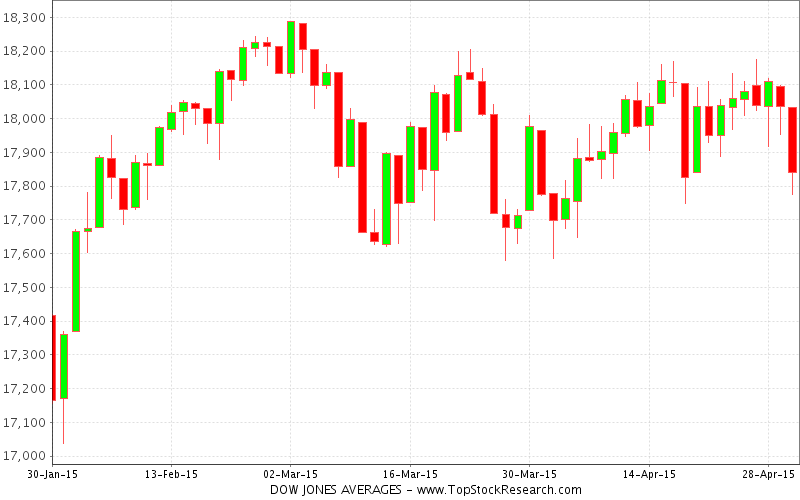
\includegraphics[width=1.0\textwidth]{img/candlestick-chart.png}
\label{figure:candlestick-chart}
\end{figure}

As mentioned before, Japanese traders noticed patterns that emerged in the candlestick charts. These patterns helped the traders to understand the current situation of a financial market and to take decisions based on these assumptions. Some example patterns are shown in Figure \ref{figure:candlestick-patterns}. For example, if a "bullish engulfing" or a "rising sun" candlestick pattern appears in the chart of a market, this is considered as a sign of a following uptrend -- which means that prices will increase. In contrast, if a "bearish engulfing" or "dark cloud cover" candlestick pattern appears, this signs a following downtrend -- which means that prices will decrease. Additionally, there are patterns that indicate that a market will start stagnating, such as the "harami" candlestick pattern. It is worth noting that these candlestick patterns are still used in modern trading strategies.

All the processes described above can be performed manually, i.e. a trader can look at price charts and start identifying candlestick patterns, draw moving averages over the chart, decide on the number of units to buy or sell, decide on take profit and stop loss levels, etc. However, with the introduction of computers to the financial world in the mid 20th century, automated or algorithmic trading was also introduced. % Amaury: \cite
Algorithmic trading help traders to partially or totally delegate trading tasks to computer software, where buy or sell transactions occur when a set of conditions are met. In this thesis, an automated trading strategy is part of the proposed method.

\begin{figure}
\caption{Example of candlestick patterns}
\centering
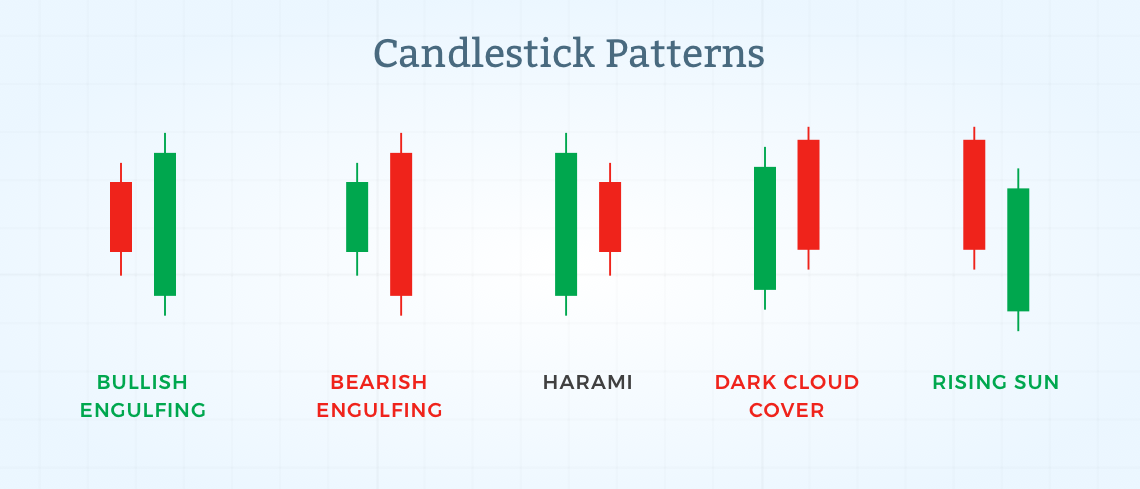
\includegraphics[width=1.0\textwidth]{img/candlestick-patterns.png}
\label{figure:candlestick-patterns}
\end{figure}

\section{Computational Intelligence}
\label{section:computational-intelligence}

Computational intelligence is a field of computer science similar to artificial intelligence. In contrast to artificial intelligence, where symbolic logic is used to represent reasoning, computational intelligence relies on statistical and bio-inspired approaches. As the models generated by computational intelligence are often not exact, but rather an approximation to the problem it is modelling, it is sometimes also called soft computing. %% Amaury: \cite

The following Sections discuss the computational intelligence techniques that are used in the proposed method of this thesis.

\subsection{Fuzzy Sets}
\label{subsection:fuzzy-sets}

A traditional set is a collection of items that share a common characteristic. This characteristic serves as a membership, because all the items in a universe either have that characteristic -- and then the item is part of the set -- or it does not have it -- and then the item is not part of the set. Traditional sets can be extended to fuzzy sets, as explained by Zadeh \cite{Zadeh1965}. Fuzzy sets are then a generalization of traditional sets, i.e. any traditional set can be represented as a fuzzy set. The difference between these two type of sets lies in the concept of membership: memberships are not only used to represent binary outcomes, i.e. \textit{true} or \textit{false}, but now a possibly infinite number of outcomes. An item can now be partially a member of a set, and the only way an item is not part of such set is if its membership is totally \textit{false}. In order to represent this grade of membership one can use real numbers. Thus, one can say, for example, that an item is \textit{0.7 green}, \textit{0.5 blue} and \textit{0.0 red}. These values can represent an adverb and an adjective, such as "very green," "somewhat blue" and "not red at all." This is especially useful when designing fuzzy systems (see Subsection \ref{subsection:fuzzy-systems}).

\subsection{Fuzzy Systems}
\label{subsection:fuzzy-systems}

In traditional logic one can generate logical inferences, such as \textit{if it's raining, then there are clouds in the sky}. In a similar fashion, one can use fuzzy sets to represent the antecedents and consequents in a logical inference process. For example, one can extend the previous example to: \textit{if it's raining a lot, then there are many clouds in the sky}.

There is a number of ways in which one can construct a fuzzy inference system, where one or more inputs or antecedents can be used to generate one or more outputs or consequents. Arguably, the two most popular types of fuzzy inference systems are the ones created by Mamdani and Assilian \cite{Mamdani1975}, and Takagi and Sugeno \cite{Takagi1985}. These systems use a series of fuzzy sets to represent the relationship between an input and its grade of membership to a set. These sets usually represent adjectives that describe the inputs, and are also considered to be the antecedents in the fuzzy inference system. For example, an input of 0.8 can represent a "very high" value. After obtaining these grades of membership, one can use these values to "fire" or "activate" the consequents. In the case of a Mamdani system, the consequents are represented as fuzzy sets, just like the antecedents. In contrast, in a Sugeno system, consequents are represented by mathematical functions. A set of rules is used to determine the relationship between the antecedents and the consequents, for example: \textit{if food quality is high then tip is high}. The aforementioned rule is creating a relationship between the fuzzy set that represents "high food quality" in the antecedents, and the fuzzy set that represents "high tip" in the consequents. Further continuing with the example, if "food quality" is represented by a value of 0.8, the rule that creates the relationship between "food quality" and "tip" could determine a "tip" of 0.8 too, depending on what membership function and what parameters are decided to be used to represent each.

It has been explained how a relationship between antecedents and consequents can be constructed in a fuzzy inference system. Nevertheless, the most interesting problem arises when a problem involves several fuzzy sets to represent different adjectives for single antecedents or consequents. In these cases, depending on the fuzzy rules, a number of consequents can be fired according to the inputs to the system. As seen in Figure \ref{figure:antecedents}, the input -- represented by the dotted vertical black line -- is associated with three fuzzy triangular sets or antecedents, where it "activates" two of them. According to a set of fuzzy rules, it then fires a set of triangular fuzzy sets that represent the consequents, as seen in Figure \ref{figure:consequents}.

The fuzzy sets that represent the consequents are cut, and new shapes are obtained using those cuts, as represented by the green shapes in Figure \ref{figure:consequents}. These shapes are aggregated and result in the output of the fuzzy inference system, and this result can then be defuzzified using different methods, such as obtaining the centroid of the shape. In this example, a Mamdani fuzzy inference system is considered; in the case of a Sugeno system, for example, the antecedents would be represented by arbitrary mathematical functions, instead of membership functions representing shapes such as the triangles in the example presented above.

\begin{figure}
\caption{Antecedents}
\centering
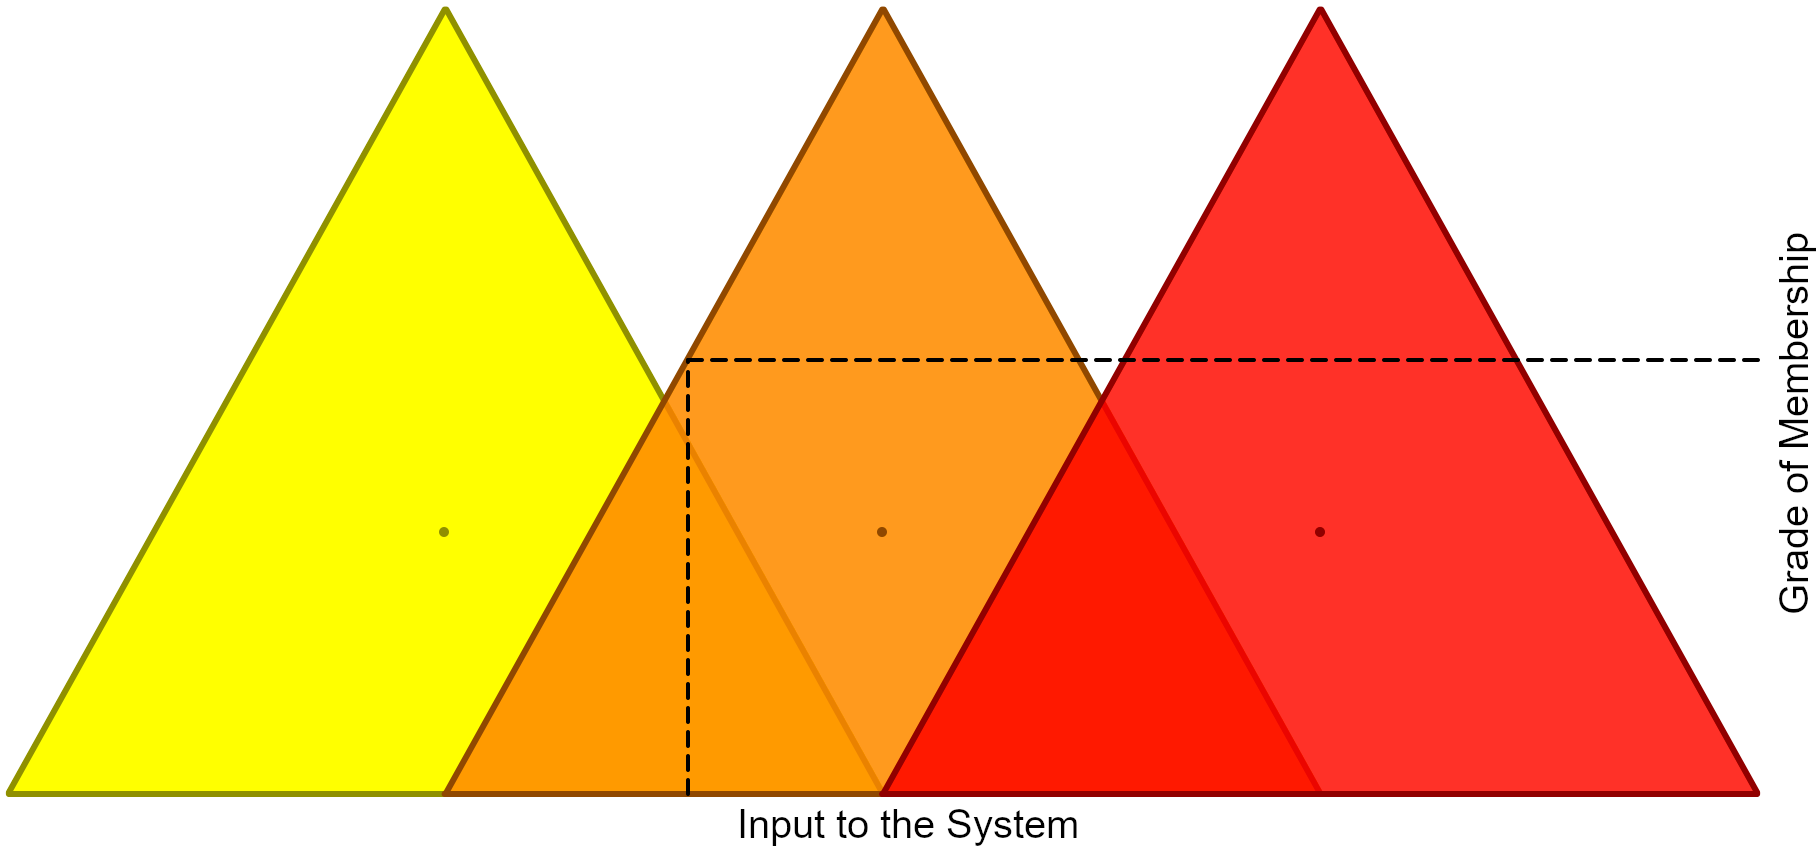
\includegraphics[width=1.0\textwidth]{img/antecedents.png}
\label{figure:antecedents}
\end{figure}

\begin{figure}
\caption{Consequents}
\centering
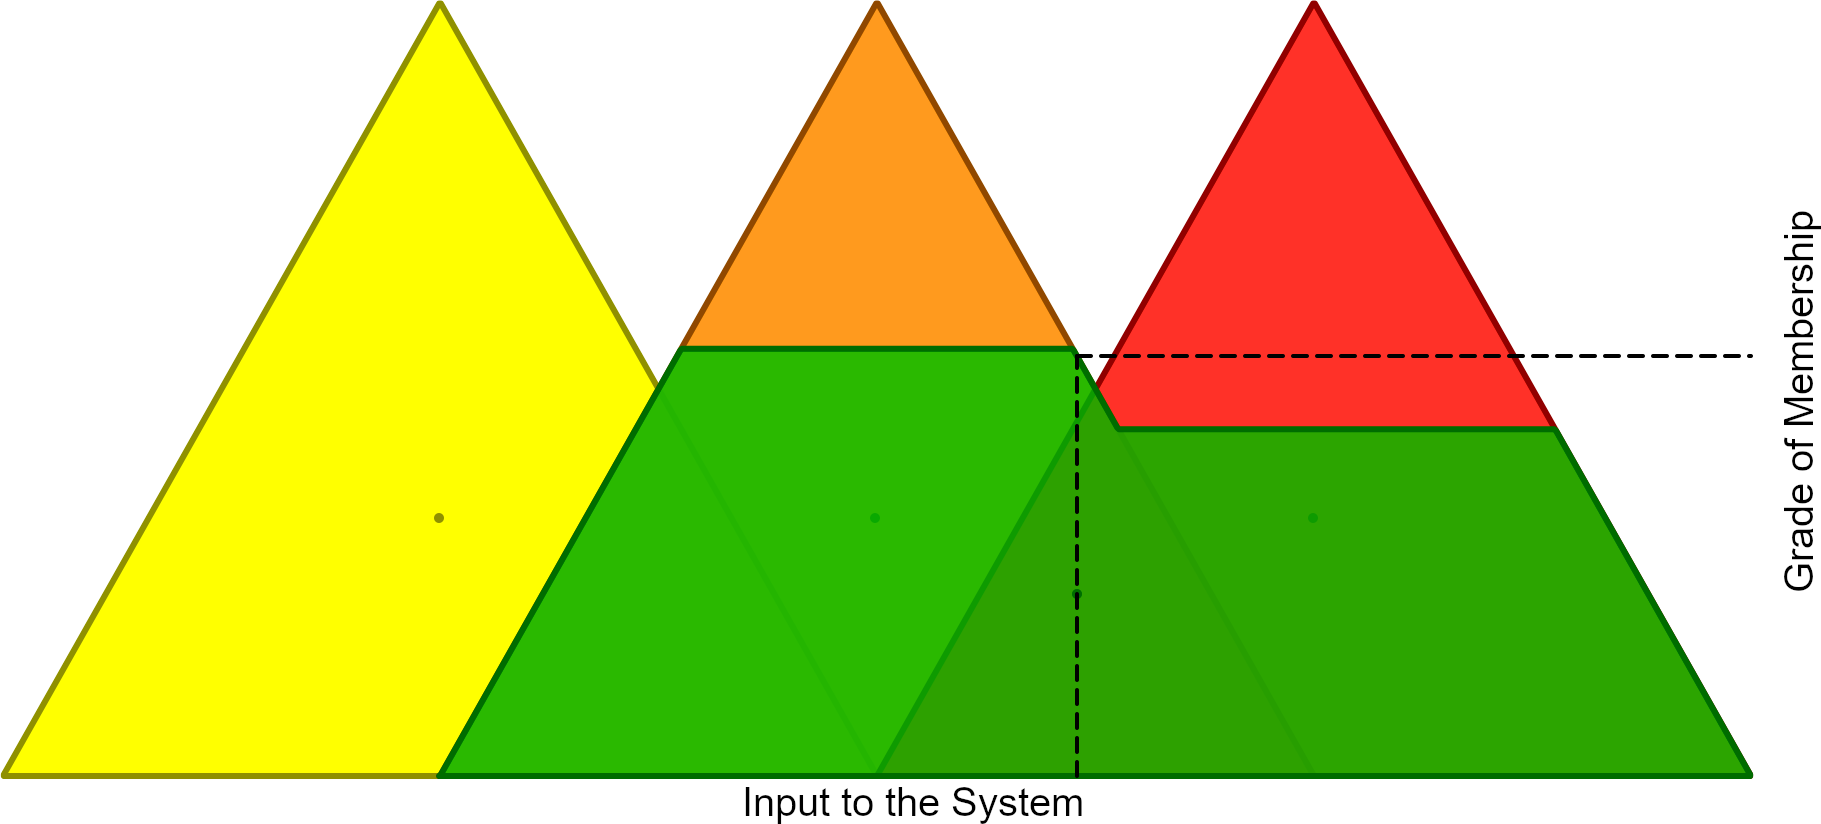
\includegraphics[width=1.0\textwidth]{img/consequents.png}
\label{figure:consequents}
\end{figure}

\subsection{Fuzzy Systems Software}
\label{subsection:fuzzy-systems-software}

There are a number of implementations of fuzzy systems toolboxes or libraries where a programmer can design a fuzzy system to be integrated with other software projects or used as stand-alone applications. The vast majority of this software is dedicated to the creation of type-1 fuzzy systems, i.e. systems that don't consider uncertainty in the grade of membership of their antecedents or consequents.

\subsection{Intuitionistic Fuzzy Sets}
\label{subsection:intuitionistic-fuzzy-sets}

In contrast to the traditional fuzzy sets discussed in Subsection \ref{subsection:fuzzy-sets}, intuitionistic fuzzy sets consider a grade of non-membership in addition to a grade of membership associated to an element in the fuzzy set, as expressed by \ref{eq:ifs-definition}.

% intuitionistic fuzzy set
\begin{equation}
  \label{eq:ifs-definition}
  A^{*} = \{\langle x, \mu _{A} (x), \nu _{A} (x) \rangle | x \in E\}
\end{equation}

For every of the elements contained in an intuitionistic fuzzy set, \ref{eq:intuitionistic-interval} must hold true.

% intuitionistic interval
\begin{equation}
  \label{eq:intuitionistic-interval}
  0 \leq \mu_{A}(x) + \nu_{A}(x) \leq 1
\end{equation}

Intuitionistic fuzzy sets are an extension to traditional fuzzy sets, as any traditional fuzzy set can be expressed as a particular case of an intuitionistic fuzzy set, as in \ref{eq:ifs-form}.

% every ordinary fuzzy set has the form
\begin{equation}
  \label{eq:ifs-form}
  \{ \langle x, \mu_{A}(x), 1 - \mu_{A}(x) \rangle | x \in E \}
\end{equation}

If the sum of the membership $\mu_{A}(x)$ and non-membership $\nu_{A}(x)$ of an element is less than $1$, the concept of indeterminacy or hesitancy arises, which is described by \ref{eq:indeterminacy}. Indeterminacy is used to represent doubt in the grade of membership of an element in an intuitionistic fuzzy set and is described by \ref{eq:indeterminacy}.

% if
\begin{equation}
  \label{eq:indeterminacy}
  \pi_{A}(x) = 1 - \mu_{A}(x) - \nu_{A}(x)
\end{equation}

Traditional fuzzy sets can be extended to increase their capabilities of representing uncertainty by introducing the concept of footprint of uncertainty. A footprint of uncertainty is achieved by extending the membership function, where each of its values are now fuzzy sets themselves, instead of crisp values. Indeterminacy serves a different purpose than the one of footprint of uncertainty. Instead of extending the uncertainty provided by traditional fuzzy sets, indeterminacy helps to model doubt. For example, if traditional fuzzy sets can model the following sentence: "the object is very hot", indeterminacy can model "it is unsure that the object is very hot".

\subsection{Intuitionistic Fuzzy Systems}
\label{subsection:intuitionistic-fuzzy-systems}

Human beings tend to express their knowledge using natural language and certain words describe abstract objects or experiences in fuzzy terms. For example, after generating a financial report, one is interested in knowing if an organization is ”doing well,” or if it is ”not profitable enough.” The previous examples are fuzzy statements that need to be inferred from data, but this data can also be uncertain (e.g. noise is present in the data). For that reason, fuzzy sets have been proposed for data modeling and knowledge representation. On the other hand, fuzzy inference systems (FIS) have been applied in the construction of control and pattern recognition systems also based on such fuzzy data. Nevertheless, occasionally there are situations where a traditional FIS can not properly model certaindatasets,duetohighlevelsofuncertaintypresentinthe data (e.g., noise). As a consequence, researchers have extended fuzzy sets and fuzzy logic theory to allow the construction of systems that can successfully represent this noisy data. One of the extensions to fuzzy sets are type-2 fuzzy sets [1]. The idea behind this extension is to add uncertainty to the membership of an element to a fuzzy set. In other words, an element willhave a certaingrade of membership to afuzzy set, and this grade of membership will be represented as another fuzzy set. For example, this technique allows a fuzzy system to be more resilient to data with many outliers; it will be easier for a type-2 fuzzy system to create a generalized model of the data than a type-1 fuzzy system. Many works have incorporated type-2 fuzzy sets into their systems and have obtained a better performance when compared to their traditional or type-1 fuzzy sets counterparts [2]. Despite this increase in capabilities for handling uncertainty, type-2 fuzzy systems have the disadvantage of being significantly slower than type1 systems [3]. The reason for this penalty in performance is mainly due to how a type-2 fuzzy system is implemented, that is, the programming language used for it and what type of programming techniques were used to implement the fuzzy theory.Onewaytomitigatethisproblemistorestrictthefuzzy sets that represent the grade of membership for an element, in order to simplify the calculations needed for the system to generate inferences, and therefore quicken the process. Interval type-2 fuzzy systems were the result of implementing this idea, which are a particular case of general type-2 fuzzy systems. Another way is to reduce the complexity of the algorithm, such as in the case of the work from Karnik and Mendel [4]. Fuzzy sets can also be extended to intuitionistic fuzzy sets (IFS), which are proposed by Atanassov in [5]. As in the case of type-2 fuzzy sets, IFS increase the capabilities of a traditional fuzzy set to represent uncertainty, by introducing the concept of indeterminacy. Basically an element that belongs to an IFS is described by a grade of membership (µ) and a grade of non-membership (ν). One can express how well an element belongs to a fuzzy set and how well an element does not belong to that fuzzy set as well. As a consequence, the sum of the values for the membership and non-membership are not always equal to 1, and 1−(µ + ν) will be known as indeterminacy, which is represented by the symbol π. FISs that implement intuitionistic fuzzy sets have at least two advantages: 1) they can handle more uncertainty than traditional FISs and can process their inferences to crisp values with almost no resource performance impact, and 2) they can still be extended to use type-2 fuzzy sets, giving as a result an intuitionistic type-2 FIS.

The use of intuitionistic fuzzy sets (IFSs) in a traditional fuzzy inference system (FIS) should enable the handling of more uncertainty, and one could prefer an intuitionistic FIS (IFIS) to obtain better accuracies without sacrificing time performance, as inferences in a type-2 FIS (T2-FIS) are very time consuming compared to a type-1 FIS (T1-FIS). This is a consequence of the complex type reducing procedure that is involved in the defuzzification stage in a T2-FIS [1]. Several improvements to the algorithms involved in the inference process in a T2-FIS have been proposed to alleviate this problem, such as the Karnik-Mendel algorithm [2] and shadowed sets [3]. Nevertheless, a T2-FIS is usually several times slower than a T1-FIS. Because of this time performance impact, many works that require handling more uncertainty than a T1-FIS use a particular case of T2-FIS, the interval T2-FIS (IT2-FIS) [4], which is faster than a general T2-FIS (GT2-FIS).Atype-1IFIS(T1-IFIS)shouldperformbetterthan a T1-FIS in terms of accuracy (in problems involving data with high levels of uncertainty), and should be faster than a T2-FIS. Furthermore, IFSs can be implemented as part of a T2-FIS, giving as a result a type-2 IFIS.

\subsection{Membership and Non-Membership Functions Design}
\label{subsection:membership-and-non-membership-functions-design}

The most common approach to graphically representing an IFS is by lattices. Examples of this type of representation can be found in the works by I. Despi et al. [12], and G. Deschrijver et al. [11]. This is a popular approach to graphically represent an IFS as it enables more compact and concise mathematical expressions. Another representation that is suitable for mathematical processes is that of a matrix, and is discussed in detail in the works by R. Parvathi et al. [16],  G. Çuvalcioglu et al. [9], and S. Yilmaz et al. [22].

IFSs have been graphically represented like membership functions are ussually represented in Mamdani FISs, and some example works are the ones by P. Angelov [2], K. T. Atanassov [4], and H. Davarzani and M. A. Khorheh [10]. This notation can be suitable for representing an architecture of an IFIS, but if the plot is in black and white, or in greyscale, the reader can get confused by the membership and non-membership plots. This problem can be alleviated by plotting the membership and non-membership functions in separate plots, is in the works by O. Castillo et al. [7], and M. Akram et al. [1].

There are several other graphical representations of IFSs, such as by radar charts, as in the work by V. Atanassova [5], and by geometrical representations, orthogonal projections and three-dimensional representations, as can be found in the work by E Szmidt and J. Kacprzyk [19].

Some applications of IFSs in the area of medical sciences can be found in the works by E. Szmidt and J. Kacprzyk [20],  C. M. Own [15], and D. D. Chakarska and L. S. Antonov [8]. In the area of group decision making, we have an example in the work by Z. Xu [21]. IFSs have also been used in word recognition, in the area of artificial vision, as in the example work of L. Baccour et al. [6].

This work proposes that IFSs, in a Mamdani IFIS, should follow an approach similar to that found in the work by K. T. Atanassov [4], where the membership is plotted as is commonly done in a traditional FIS, but the non-membership function should be plotted as 1-υA. The reason behind this decision is that the non-membership function should be easily differentiated from the membership function, while seeing both functions in the same plot. An implementation of an IFIS that uses this approach for representing IFSs for a Mamdani IFIS can be found in the work by A. Hernandez-Aguila and M. Garcia-Valdez [13].

In Figure \ref{figure:traditional-set-as-ifs}, one can see how a traditional fuzzy set can be constructed using the proposed approach. A Gaussian membership function with mean of 50 and a standard deviation of 15 is depicted.


\begin{figure}
\caption{A traditional fuzzy set represented as an intuitionistic fuzzy set}
\centering
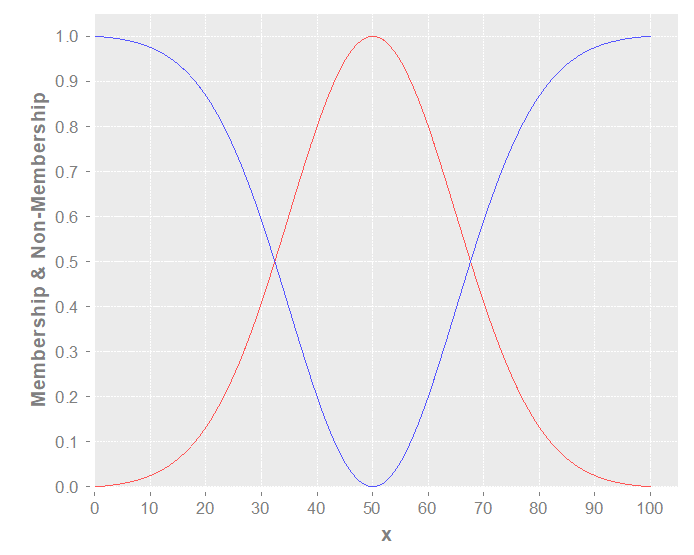
\includegraphics[width=1.0\textwidth]{img/traditional-set-as-ifs.png}
\label{figure:traditional-set-as-ifs}
\end{figure}

Figure \ref{figure:example-of-ifs} is the first case of an IFS that cannot be considered a tradi-tional fuzzy set. The red line represents the membership function, while the blue line represents the non-membership function. As can be seen, the Gaussian membership function does not have a kernel, meaning that its highest valued member does not equal to 1. In this case, its highest valued member equals to 0.7, and for the non-membership function, its highest valued member equals to 0.3. The Gaussian membership function is constructed with a mean of 50 and a standard deviation of 15. For the non-membership function, it is con-structed with a mean of 30 and standard deviation of 30.

\begin{figure}
\caption{Representation of an intuitionistic fuzzy set}
\centering
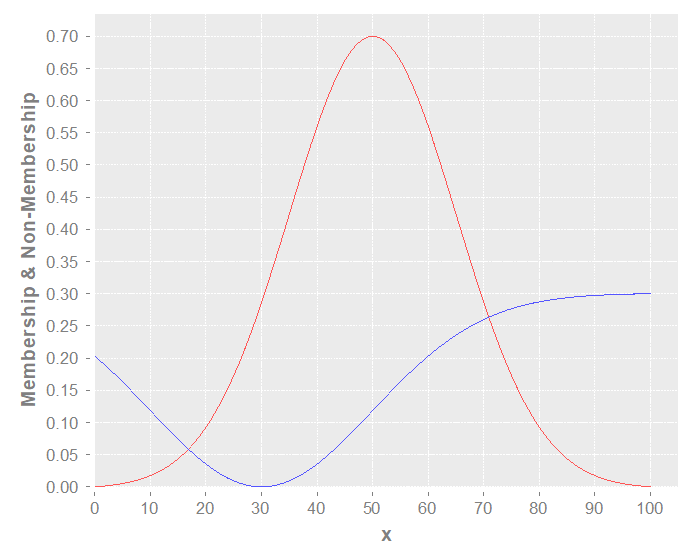
\includegraphics[width=1.0\textwidth]{img/example-of-ifs.png}
\label{figure:example-of-ifs}
\end{figure}

\subsection{Genetic Algorithms}
\label{subsection:genetic-algorithms}

\section{Multi-agent Systems and Models}
\label{section:multi-agent-systems-and-models}

\section{Technical Analysis}
\label{section:technical-analysis}

\section{Retracements in Financial Markets}
\label{section:retracements-in-financial-markets}

